
%% bare_conf.tex
%% V1.4b
%% 2015/08/26
%% by Michael Shell
%% See:
%% http://www.michaelshell.org/
%% for current contact information.
%%
%% This is a skeleton file demonstrating the use of IEEEtran.cls
%% (requires IEEEtran.cls version 1.8b or later) with an IEEE
%% conference paper.
%%
%% Support sites:
%% http://www.michaelshell.org/tex/ieeetran/
%% http://www.ctan.org/pkg/ieeetran
%% and
%% http://www.ieee.org/

%%*************************************************************************
%% Legal Notice:
%% This code is offered as-is without any warranty either expressed or
%% implied; without even the implied warranty of MERCHANTABILITY or
%% FITNESS FOR A PARTICULAR PURPOSE! 
%% User assumes all risk.
%% In no event shall the IEEE or any contributor to this code be liable for
%% any damages or losses, including, but not limited to, incidental,
%% consequential, or any other damages, resulting from the use or misuse
%% of any information contained here.
%%
%% All comments are the opinions of their respective authors and are not
%% necessarily endorsed by the IEEE.
%%
%% This work is distributed under the LaTeX Project Public License (LPPL)
%% ( http://www.latex-project.org/ ) version 1.3, and may be freely used,
%% distributed and modified. A copy of the LPPL, version 1.3, is included
%% in the base LaTeX documentation of all distributions of LaTeX released
%% 2003/12/01 or later.
%% Retain all contribution notices and credits.
%% ** Modified files should be clearly indicated as such, including  **
%% ** renaming them and changing author support contact information. **
%%*************************************************************************


% *** Authors should verify (and, if needed, correct) their LaTeX system  ***
% *** with the testflow diagnostic prior to trusting their LaTeX platform ***
% *** with production work. The IEEE's font choices and paper sizes can   ***
% *** trigger bugs that do not appear when using other class files.       ***                          ***
% The testflow support page is at:
% http://www.michaelshell.org/tex/testflow/



\documentclass[conference]{IEEEtran}

\usepackage{graphicx}	
\usepackage{epstopdf}
\usepackage{color}
%\usepackage{subcaption}
 \usepackage{float}
 \usepackage{wrapfig}
\ifCLASSOPTIONcompsoc
  \usepackage[caption=false,font=normalsize,labelfont=sf,textfont=sf]{subfig}
\else
  \usepackage[caption=false,font=footnotesize]{subfig}
\fi


% Some Computer Society conferences also require the compsoc mode option,
% but others use the standard conference format.
%
% If IEEEtran.cls has not been installed into the LaTeX system files,
% manually specify the path to it like:
% \documentclass[conference]{../sty/IEEEtran}





% Some very useful LaTeX packages include:
% (uncomment the ones you want to load)


% *** MISC UTILITY PACKAGES ***
%
%\usepackage{ifpdf}
% Heiko Oberdiek's ifpdf.sty is very useful if you need conditional
% compilation based on whether the output is pdf or dvi.
% usage:
% \ifpdf
%   % pdf code
% \else
%   % dvi code
% \fi
% The latest version of ifpdf.sty can be obtained from:
% http://www.ctan.org/pkg/ifpdf
% Also, note that IEEEtran.cls V1.7 and later provides a builtin
% \ifCLASSINFOpdf conditional that works the same way.
% When switching from latex to pdflatex and vice-versa, the compiler may
% have to be run twice to clear warning/error messages.






% *** CITATION PACKAGES ***
%
%\usepackage{cite}
% cite.sty was written by Donald Arseneau
% V1.6 and later of IEEEtran pre-defines the format of the cite.sty package
% \cite{} output to follow that of the IEEE. Loading the cite package will
% result in citation numbers being automatically sorted and properly
% "compressed/ranged". e.g., [1], [9], [2], [7], [5], [6] without using
% cite.sty will become [1], [2], [5]--[7], [9] using cite.sty. cite.sty's
% \cite will automatically add leading space, if needed. Use cite.sty's
% noadjust option (cite.sty V3.8 and later) if you want to turn this off
% such as if a citation ever needs to be enclosed in parenthesis.
% cite.sty is already installed on most LaTeX systems. Be sure and use
% version 5.0 (2009-03-20) and later if using hyperref.sty.
% The latest version can be obtained at:
% http://www.ctan.org/pkg/cite
% The documentation is contained in the cite.sty file itself.






% *** GRAPHICS RELATED PACKAGES ***
%
\ifCLASSINFOpdf
  % \usepackage[pdftex]{graphicx}
  % declare the path(s) where your graphic files are
  % \graphicspath{{../pdf/}{../jpeg/}}
  % and their extensions so you won't have to specify these with
  % every instance of \includegraphics
  % \DeclareGraphicsExtensions{.pdf,.jpeg,.png}
\else
  % or other class option (dvipsone, dvipdf, if not using dvips). graphicx
  % will default to the driver specified in the system graphics.cfg if no
  % driver is specified.
  % \usepackage[dvips]{graphicx}
  % declare the path(s) where your graphic files are
  % \graphicspath{{../eps/}}
  % and their extensions so you won't have to specify these with
  % every instance of \includegraphics
  % \DeclareGraphicsExtensions{.eps}
\fi
% graphicx was written by David Carlisle and Sebastian Rahtz. It is
% required if you want graphics, photos, etc. graphicx.sty is already
% installed on most LaTeX systems. The latest version and documentation
% can be obtained at: 
% http://www.ctan.org/pkg/graphicx
% Another good source of documentation is "Using Imported Graphics in
% LaTeX2e" by Keith Reckdahl which can be found at:
% http://www.ctan.org/pkg/epslatex
%
% latex, and pdflatex in dvi mode, support graphics in encapsulated
% postscript (.eps) format. pdflatex in pdf mode supports graphics
% in .pdf, .jpeg, .png and .mps (metapost) formats. Users should ensure
% that all non-photo figures use a vector format (.eps, .pdf, .mps) and
% not a bitmapped formats (.jpeg, .png). The IEEE frowns on bitmapped formats
% which can result in "jaggedy"/blurry rendering of lines and letters as
% well as large increases in file sizes.
%
% You can find documentation about the pdfTeX application at:
% http://www.tug.org/applications/pdftex





% *** MATH PACKAGES ***
%
%\usepackage{amsmath}
% A popular package from the American Mathematical Society that provides
% many useful and powerful commands for dealing with mathematics.
%
% Note that the amsmath package sets \interdisplaylinepenalty to 10000
% thus preventing page breaks from occurring within multiline equations. Use:
%\interdisplaylinepenalty=2500
% after loading amsmath to restore such page breaks as IEEEtran.cls normally
% does. amsmath.sty is already installed on most LaTeX systems. The latest
% version and documentation can be obtained at:
% http://www.ctan.org/pkg/amsmath





% *** SPECIALIZED LIST PACKAGES ***
%
%\usepackage{algorithmic}
% algorithmic.sty was written by Peter Williams and Rogerio Brito.
% This package provides an algorithmic environment fo describing algorithms.
% You can use the algorithmic environment in-text or within a figure
% environment to provide for a floating algorithm. Do NOT use the algorithm
% floating environment provided by algorithm.sty (by the same authors) or
% algorithm2e.sty (by Christophe Fiorio) as the IEEE does not use dedicated
% algorithm float types and packages that provide these will not provide
% correct IEEE style captions. The latest version and documentation of
% algorithmic.sty can be obtained at:
% http://www.ctan.org/pkg/algorithms
% Also of interest may be the (relatively newer and more customizable)
% algorithmicx.sty package by Szasz Janos:
% http://www.ctan.org/pkg/algorithmicx




% *** ALIGNMENT PACKAGES ***
%
%\usepackage{array}
% Frank Mittelbach's and David Carlisle's array.sty patches and improves
% the standard LaTeX2e array and tabular environments to provide better
% appearance and additional user controls. As the default LaTeX2e table
% generation code is lacking to the point of almost being broken with
% respect to the quality of the end results, all users are strongly
% advised to use an enhanced (at the very least that provided by array.sty)
% set of table tools. array.sty is already installed on most systems. The
% latest version and documentation can be obtained at:
% http://www.ctan.org/pkg/array


% IEEEtran contains the IEEEeqnarray family of commands that can be used to
% generate multiline equations as well as matrices, tables, etc., of high
% quality.




% *** SUBFIGURE PACKAGES ***
%\ifCLASSOPTIONcompsoc
%  \usepackage[caption=false,font=normalsize,labelfont=sf,textfont=sf]{subfig}
%\else
%  \usepackage[caption=false,font=footnotesize]{subfig}
%\fi
% subfig.sty, written by Steven Douglas Cochran, is the modern replacement
% for subfigure.sty, the latter of which is no longer maintained and is
% incompatible with some LaTeX packages including fixltx2e. However,
% subfig.sty requires and automatically loads Axel Sommerfeldt's caption.sty
% which will override IEEEtran.cls' handling of captions and this will result
% in non-IEEE style figure/table captions. To prevent this problem, be sure
% and invoke subfig.sty's "caption=false" package option (available since
% subfig.sty version 1.3, 2005/06/28) as this is will preserve IEEEtran.cls
% handling of captions.
% Note that the Computer Society format requires a larger sans serif font
% than the serif footnote size font used in traditional IEEE formatting
% and thus the need to invoke different subfig.sty package options depending
% on whether compsoc mode has been enabled.
%
% The latest version and documentation of subfig.sty can be obtained at:
% http://www.ctan.org/pkg/subfig




% *** FLOAT PACKAGES ***
%
%\usepackage{fixltx2e}
% fixltx2e, the successor to the earlier fix2col.sty, was written by
% Frank Mittelbach and David Carlisle. This package corrects a few problems
% in the LaTeX2e kernel, the most notable of which is that in current
% LaTeX2e releases, the ordering of single and double column floats is not
% guaranteed to be preserved. Thus, an unpatched LaTeX2e can allow a
% single column figure to be placed prior to an earlier double column
% figure.
% Be aware that LaTeX2e kernels dated 2015 and later have fixltx2e.sty's
% corrections already built into the system in which case a warning will
% be issued if an attempt is made to load fixltx2e.sty as it is no longer
% needed.
% The latest version and documentation can be found at:
% http://www.ctan.org/pkg/fixltx2e


%\usepackage{stfloats}
% stfloats.sty was written by Sigitas Tolusis. This package gives LaTeX2e
% the ability to do double column floats at the bottom of the page as well
% as the top. (e.g., "\begin{figure*}[!b]" is not normally possible in
% LaTeX2e). It also provides a command:
%\fnbelowfloat
% to enable the placement of footnotes below bottom floats (the standard
% LaTeX2e kernel puts them above bottom floats). This is an invasive package
% which rewrites many portions of the LaTeX2e float routines. It may not work
% with other packages that modify the LaTeX2e float routines. The latest
% version and documentation can be obtained at:
% http://www.ctan.org/pkg/stfloats
% Do not use the stfloats baselinefloat ability as the IEEE does not allow
% \baselineskip to stretch. Authors submitting work to the IEEE should note
% that the IEEE rarely uses double column equations and that authors should try
% to avoid such use. Do not be tempted to use the cuted.sty or midfloat.sty
% packages (also by Sigitas Tolusis) as the IEEE does not format its papers in
% such ways.
% Do not attempt to use stfloats with fixltx2e as they are incompatible.
% Instead, use Morten Hogholm'a dblfloatfix which combines the features
% of both fixltx2e and stfloats:
%
% \usepackage{dblfloatfix}
% The latest version can be found at:
% http://www.ctan.org/pkg/dblfloatfix




% *** PDF, URL AND HYPERLINK PACKAGES ***
%
%\usepackage{url}
% url.sty was written by Donald Arseneau. It provides better support for
% handling and breaking URLs. url.sty is already installed on most LaTeX
% systems. The latest version and documentation can be obtained at:
% http://www.ctan.org/pkg/url
% Basically, \url{my_url_here}.




% *** Do not adjust lengths that control margins, column widths, etc. ***
% *** Do not use packages that alter fonts (such as pslatex).         ***
% There should be no need to do such things with IEEEtran.cls V1.6 and later.
% (Unless specifically asked to do so by the journal or conference you plan
% to submit to, of course. )


% correct bad hyphenation here
\hyphenation{op-tical net-works semi-conduc-tor}


\begin{document}
%
% paper title
% Titles are generally capitalized except for words such as a, an, and, as,
% at, but, by, for, in, nor, of, on, or, the, to and up, which are usually
% not capitalized unless they are the first or last word of the title.
% Linebreaks \\ can be used within to get better formatting as desired.
% Do not put math or special symbols in the title.
\title{Project 1 for Complex Adaptive Systems}


% author names and affiliations
% use a multiple column layout for up to three different
% affiliations
\author{\IEEEauthorblockN{Vanessa Job}
\IEEEauthorblockA{Department of Computer Science\\
University of New Mexico\\
\
vjob@unm.edu}
\and
\IEEEauthorblockN{Kellin Rumsey}
\IEEEauthorblockA{Department of Mathematics and Statistics\\
University of New Mexico\\
knrumsey@unm.edu}
}

% conference papers do not typically use \thanks and this command
% is locked out in conference mode. If really needed, such as for
% the acknowledgment of grants, issue a \IEEEoverridecommandlockouts
% after \documentclass

% for over three affiliations, or if they all won't fit within the width
% of the page, use this alternative format:
% 
%\author{\IEEEauthorblockN{Michael Shell\IEEEauthorrefmark{1},
%Homer Simpson\IEEEauthorrefmark{2},
%James Kirk\IEEEauthorrefmark{3}, 
%Montgomery Scott\IEEEauthorrefmark{3} and
%Eldon Tyrell\IEEEauthorrefmark{4}}
%\IEEEauthorblockA{\IEEEauthorrefmark{1}School of Electrical and Computer Engineering\\
%Georgia Institute of Technology,
%Atlanta, Georgia 30332--0250\\ Email: see http://www.michaelshell.org/contact.html}
%\IEEEauthorblockA{\IEEEauthorrefmark{2}Twentieth Century Fox, Springfield, USA\\
%Email: homer@thesimpsons.com}
%\IEEEauthorblockA{\IEEEauthorrefmark{3}Starfleet Academy, San Francisco, California 96678-2391\\
%Telephone: (800) 555--1212, Fax: (888) 555--1212}
%\IEEEauthorblockA{\IEEEauthorrefmark{4}Tyrell Inc., 123 Replicant Street, Los Angeles, California 90210--4321}}




% use for special paper notices
%\IEEEspecialpapernotice{(Invited Paper)}




% make the title area
\maketitle

% As a general rule, do not put math, special symbols or citations
% in the abstract
\begin{abstract}
The abstract goes here.
\end{abstract}

% no keywords




% For peer review papers, you can put extra information on the cover
% page as needed:
% \ifCLASSOPTIONpeerreview
% \begin{center} \bfseries EDICS Category: 3-BBND \end{center}
% \fi
%
% For peerreview papers, this IEEEtran command inserts a page break and
% creates the second title. It will be ignored for other modes.
\IEEEpeerreviewmaketitle



\section{Introduction}
% no \IEEEPARstart
\noindent Evolution proceeds by emergence of new higher level entities.   How information is stored and processed is a driver of this process \cite{Walker}.   For instance, the emergence of epigenetic inheritance provided a competitive advantage through diversification.  
In this paper, we look at the interaction between organisms as individual  populations and organisms considered as a group of populations. \\ 

\noindent For individual populations, we assume birth rate, death rate, and  carrying capacity are all fixed.  Define $k$ to be the carrying capacity of a population and $n_t$ to be size of the population at time $t$. Then the size of the population at generation $t$ is modeled by 
\begin{eqnarray}
n_{t+1} = (\textnormal{birthrate} - \textnormal{deathrate}) (k n_t - n_t^2) / k 
\end{eqnarray}
If we define the population size relative to the carrying capacity as  $x_t = n_t / k$ and define the reproductive fitness  $r = birthrate - deathrate$.  Then we  get the following equation for $x_t$: 
\begin{eqnarray}
x(t+1) = x_{t+1} = r  x_t (1 - x_t), \ \ \ \ \  t=0, 1, 2, \ldots . 
\label{logistic}
\end{eqnarray}
This is the logistic map as defined in \cite{Mitchell}.  In what follows, we will refer to $x_t$ as the population size, with the understanding that it will always be the ratio of the actual population size to the carrying capacity

In \cite{Walker}, the authors investigate information flow between higher and lower levels of organization, between individuals of a population and the population considered as a whole. 
They study a model that consists of a population of individual populations and examine the direction of the causal information transfer, where 
"non-trivial collective behavior is associated with the degree to which local elements receive information from the global network." \cite{Walker}

Their model, a lattice of  globally coupled logistic maps, is used to investigate the circumstances under which nontrivial collective behavior occurs . It shows how a reversal in the dominant direction of information flow from bottom-up to top-down is correlated with the emergence of collective behavior of the populations.  

{\it FROM INSTRUCTIONS One to two paragraphs that summarize the purpose, methods and analysis of the Walker paper and how you extend that analysis. }


KELLIN:  State HOW DO WE EXTEND THIS ANALYSIS?  


% You must have at least 2 lines in the paragraph with the drop letter
% (should never be an issue)


% \subsection{Subsection Heading Here}
% Subsection text here.


% An example of a floating figure using the graphicx package.
% Note that \label must occur AFTER (or within) \caption.
% For figures, \caption should occur after the \includegraphics.
% Note that IEEEtran v1.7 and later has special internal code that
% is designed to preserve the operation of \label within \caption
% even when the captionsoff option is in effect. However, because
% of issues like this, it may be the safest practice to put all your
% \label just after \caption rather than within \caption{}.
%
% Reminder: the "draftcls" or "draftclsnofoot", not "draft", class
% option should be used if it is desired that the figures are to be
% displayed while in draft mode.
%
%\begin{figure}[!t]
%\centering
%\includegraphics[width=2.5in]{myfigure}
% where an .eps filename suffix will be assumed under latex, 
% and a .pdf suffix will be assumed for pdflatex; or what has been declared
% via \DeclareGraphicsExtensions.
%\caption{Simulation results for the network.}
%\label{fig_sim}
%\end{figure}

% Note that the IEEE typically puts floats only at the top, even when this
% results in a large percentage of a column being occupied by floats.


% An example of a double column floating figure using two subfigures.
% (The subfig.sty package must be loaded for this to work.)
% The subfigure \label commands are set within each subfloat command,
% and the \label for the overall figure must come after \caption.
% \hfil is used as a separator to get equal spacing.
% Watch out that the combined width of all the subfigures on a 
% line do not exceed the text width or a line break will occur.
%
%\begin{figure*}[!t]
%\centering
%\subfloat[Case I]{\includegraphics[width=2.5in]{box}%
%\label{fig_first_case}}
%\hfil
%\subfloat[Case II]{\includegraphics[width=2.5in]{box}%
%\label{fig_second_case}}
%\caption{Simulation results for the network.}
%\label{fig_sim}
%\end{figure*}
%
% Note that often IEEE papers with subfigures do not employ subfigure
% captions (using the optional argument to \subfloat[]), but instead will
% reference/describe all of them (a), (b), etc., within the main caption.
% Be aware that for subfig.sty to generate the (a), (b), etc., subfigure
% labels, the optional argument to \subfloat must be present. If a
% subcaption is not desired, just leave its contents blank,
% e.g., \subfloat[].


% An example of a floating table. Note that, for IEEE style tables, the
% \caption command should come BEFORE the table and, given that table
% captions serve much like titles, are usually capitalized except for words
% such as a, an, and, as, at, but, by, for, in, nor, of, on, or, the, to
% and up, which are usually not capitalized unless they are the first or
% last word of the caption. Table text will default to \footnotesize as
% the IEEE normally uses this smaller font for tables.
% The \label must come after \caption as always.
%
%\begin{table}[!t]
%% increase table row spacing, adjust to taste
%\renewcommand{\arraystretch}{1.3}
% if using array.sty, it might be a good idea to tweak the value of
% \extrarowheight as needed to properly center the text within the cells
%\caption{An Example of a Table}
%\label{table_example}
%\centering
%% Some packages, such as MDW tools, offer better commands for making tables
%% than the plain LaTeX2e tabular which is used here.
%\begin{tabular}{|c||c|}
%\hline
%One & Two\\
%\hline
%Three & Four\\
%\hline
%\end{tabular}
%\end{table}


% Note that the IEEE does not put floats in the very first column
% - or typically anywhere on the first page for that matter. Also,
% in-text middle ("here") positioning is typically not used, but it
% is allowed and encouraged for Computer Society conferences (but
% not Computer Society journals). Most IEEE journals/conferences use
% top floats exclusively. 
% Note that, LaTeX2e, unlike IEEE journals/conferences, places
% footnotes above bottom floats. This can be corrected via the
% \fnbelowfloat command of the stfloats package.




\section{Methods and Results}

\subsection{Sensitive Dependence on Initial Conditions for the Logistic Map}

Depending on the value of the reproductive fitness $r$, the logistic map will generate a population size that is stable, periodic, or chaotic over time.  The behavior of the logistic map can vary a great deal with small changes in $x_0$.  This phenomenon is known as {\it sensitive dependence on initial conditions}, where small changes in the input lead to large changes in the output.  In figure \ref{figure1abcd}, we plot four times series showing population versus time for $50$ time steps.   
%r, initial x values and cross entropy
% a = 0.7522
% b = 
% ab mutual information  0.7522

%cd mutual information   0.0471
The mutual information measures the dependence of one random variable on another random variable.   For two random variables $X$ and $Y$, we define the mutual information to be
\begin{eqnarray}
I(X,Y) = \sum_{y \in Y} \sum_ {x \in X} p(x,y) { \log p(x,y) \over {\log p(x)  \log p(y)} }
\end{eqnarray}
When two random variables are independent, their mutual information is $0$.  

We computed the mutual information for the time series in figure \ref{figure1abcd}(a) and figure \ref{figure1abcd}(b).  
The mutual information for the periodic maps in figure \ref{abcd_combined}(a)  is $0.7522$ and the mutual information for the chaotic maps it $0.471$.   This makes sense because after $t=13$, for the periodic maps, you can certainly determine the value one map by knowing the other.  It also makes sense that the mutual information for the chaotic maps should be close to zero because they are chaotic.  

To compute the mutual information, we produced values that could be binned by multiplying each population size by 100 and rounding to the nearest integer.  Then we used the JIDT AutoAnalyzer \cite{JIDT} to compute the mutual information.    To generate figure \ref{figure1abcd} we used Matlab \cite{Matlab} with logistic map equation from \cite{Mitchell}.  

MISSING {\it From instructions:  You might follow Flake?s suggestion of predicting how far into the future two populations are on the same side of 50\% of carrying capacity and use a binary representation. You might use JIDT?s kernel estimator. Explain your choice. }



\begin{figure}[H]
\centering
 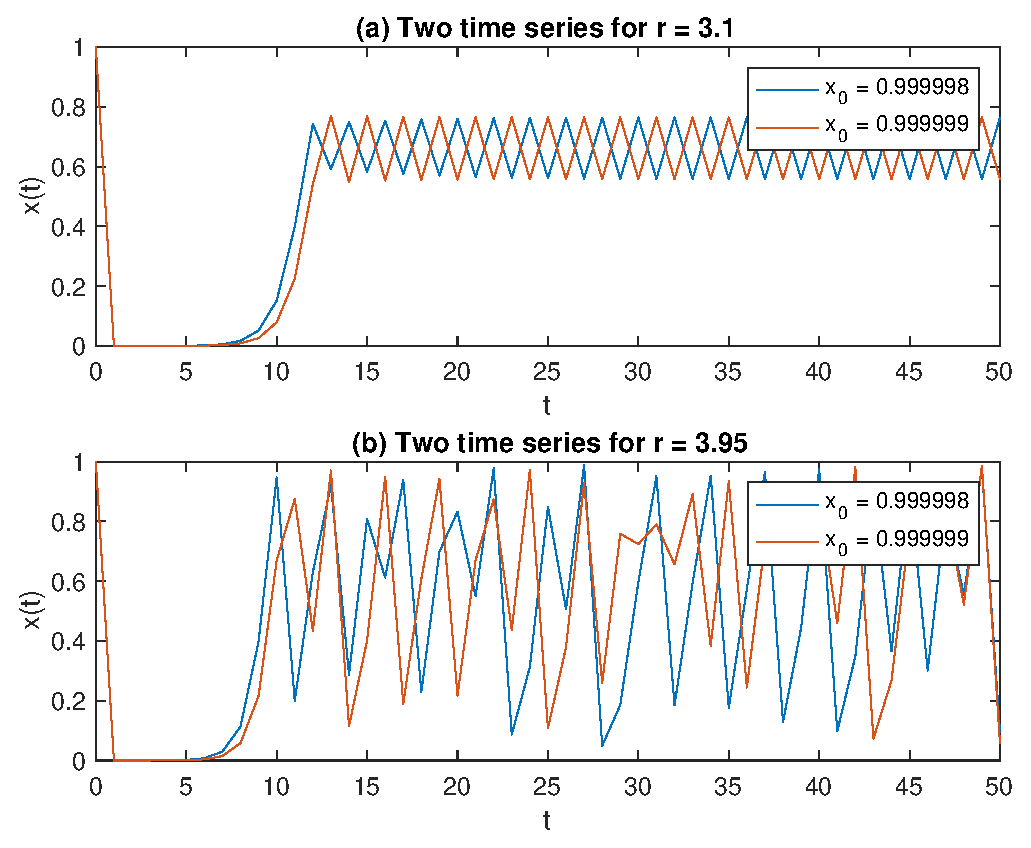
\includegraphics[width=90mm]{figure1abcd_combined}
    
  \caption{ Population growth over time showing sensitive dependence on initial conditions.  The mutual information for the periodic map (a) is 0.7522.  The mutual information for the chaotic map (b) is 0.0471.}
 \label{figure1abcd}
\end{figure} 

\subsection{The Walker Model}
For this project, we used the  model of coupled growth defined in \cite{Walker}. This model uses a logistic growth model on a lattice of populations coupled with influence from the entire population of populations.  For each time step $n$, the size of population $i$ at time step $n$ is defined to be
\begin{eqnarray}
x_{i, n+1} = (1 - \epsilon) f_i(x_{i,n}) + \epsilon m_n, \ \ \ (i=1, 2, \ldots N)
\label{coupling}
\end{eqnarray}
Here $N$ is the number of time steps, $n$ is the current time step (or generation), and $\epsilon$ is the coupling strength of the model to the entire lattice of organisms.   Here the the local growth dynamics of each population $i$ is defined by 
\begin{eqnarray}
f_i(x_{i,n}) = r_i x_{i,n} (1 - {x_{i,n} \over K})
\label{individual}
\end{eqnarray}
Here $r_i$ is the reproductive fitness of population $i$ and $K$ is the carrying capacity.    

We model the state of the entire lattice at time $n$ is an average of the states of all the populations.  This is called the instantaneous mean field and defined to be
\begin{eqnarray}
M_n = { 1 \over N} \sum _{j=1}^N x_{j,n}
\label{bigM}
\end{eqnarray}
 The mean-field $m_n$ is a measure of how the individual populations are growing at any time-step $j$.  It is defined to be 
 \begin{eqnarray}
 m_n = {1 \over N} \sum_{j=1}^N f_j(x_{j,n})
 \label{littlem}
\end{eqnarray}
The influence of $m_i$ on the entire system is quantified by the parameter $\epsilon$, the coupling strength.  
 
To do our simulation,  we set the carrying capacity $K$ to be 100 for all populations $i$, the number of populations $N = 1000$ and use $10000$ time steps.   We set the initial population size $x_i, 0$ to be $1$.   We also generated a random fitness $r_i$ for each population $i$.   

In figure \ref{prettypicture}, we show the return maps for a selection of coupling strengths $\epsilon$.  

% Figure for part 2
 \begin{figure}[H]
 \centering
    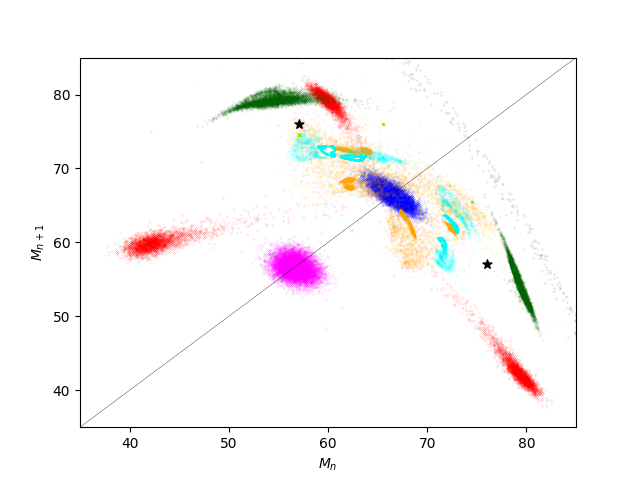
\includegraphics[width=100mm]{prettypicture}
    
    \caption{ Return map for selected values of  the global coupling strength $\epsilon$:  $\epsilon =0$ (magenta), $\epsilon = 0.075$ (red), $\epsilon = 0.1$ (blue), $\epsilon = 0.25$ (orange), $\epsilon = 0.225$ (aqua), $\epsilon = 0.25$ (dark green), $\epsilon = 3 $ (stars) and $\epsilon = 4$ (black)}
 \label{prettypicture}
\end{figure} 

To build the return map, equations \ref{coupling},  \ref{individual}, \ref{bigM},  and \ref{littlem} were implemented  in Python using Numpy \cite{numpy} and Matplotlib \cite{matplotlib}.   The return map shows that when the coupling $\epsilon = 0$,  (magenta) there is not much change in how the overall state of the populations changes from time step to time step.  That is, populations  act as isolated populations.   When $\epsilon > 0$, we see a variety of behaviors. 

It should be noted that there is quite a bit of dependence on the initial fitness values $r_i$   In different runs of the return map, $\epsilon = 0.25$ (dark green) and and $\epsilon = 0.225$ (aqua) populations sometimes form loops and there can be some scatter instead of two fixed points when $\epsilon = 0.3$.  Overall, we see that coupling strengths $0, 0.075, 0.1$ and $0.4$ produce predictably shaped regions, while there can be variation in the regions produced by $\epsilon = 0.2,  \epsilon = 0.225$ and $\epsilon = 0.3$. 

% In figure \ref{eyeglasses}, we see another possible return map.  

%\begin{figure}[H]
%\centering
  %  \includegraphics[width=100mm]{eyeglasses}
    
   % \caption{ Another return map for selected values of  the global coupling strength $\epsilon$:  $\epsilon =0$ (red), $\epsilon = 0.1$ (blue), $\epsilon = 0.25$ (orange), $\epsilon = 0.225$ (aqua), $\epsilon = 0.25$ (dark green), $\epsilon = 3 $ (stars) and $\epsilon = 4$ (black)}
 %\label{eyeglasses}
%\end{figure} 

While return maps that look like figure \ref{prettypicture} seemed to occur more often, it would be interesting to look at the distributions of fitness values $r_i$ that produce the more exotic return maps.  This is outside of the scope of this paper.
\begin{figure*}[!t]
\centering
\subfloat[]{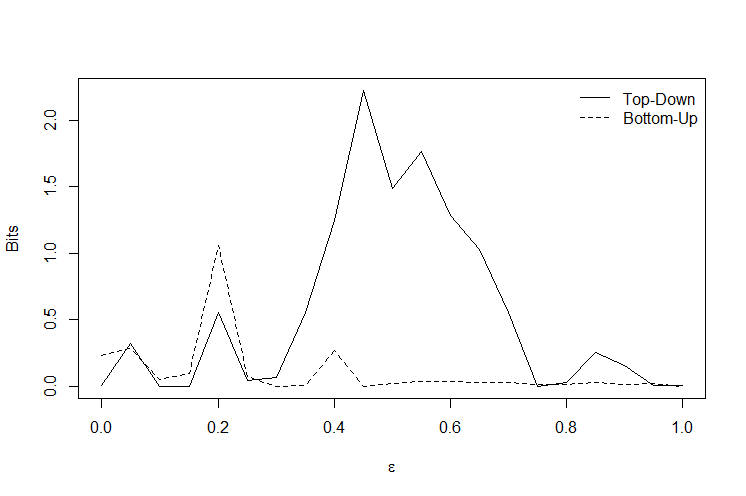
\includegraphics[width=3.5in]{Fig4a}%
\label{te}}
\hfill
\subfloat[]{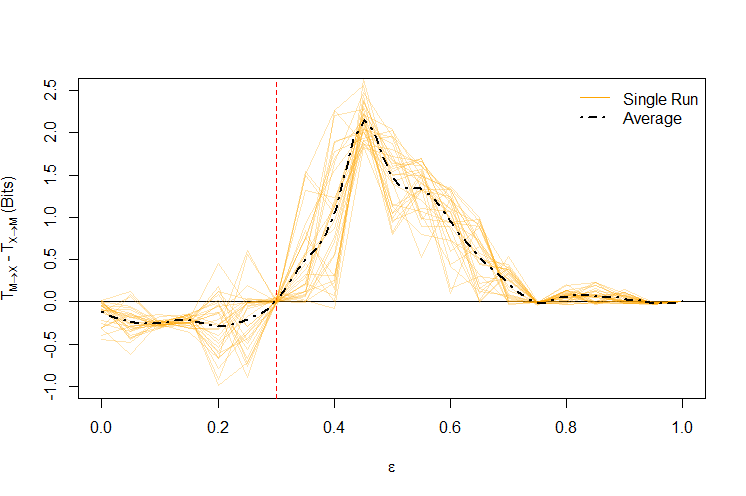
\includegraphics[width=3.5in]{Fig4b}%
\label{fig_second_case}}
\caption{Simulation results for the network.}
\label{te_avg}
\end{figure*}
\subsection{Direction of Information Flow}
\noindent In order to assess that direction of information flow, from Global to Local scales and vice versa, the authors in \cite{Walker} take advantage of {\it Transfer Entropy}. Transfer Entropy is defined mathematically in \cite{Schreiber} as
$$T^{(k)}_{Y \rightarrow X} = \sum_n p(x_{n+1}, x_n^{(k)}, y_n^{(k)}) \log \left[ \frac{p(x_{n+1}|x_n^{(k)}, y_n^{(k)})}{p(x_{n+1}|x_n{(k)}}\right]$$
Where $x_n^{(k)}$ is an embedded state in the $k$-dimensional phase spate defined as $x_n^{(k)} = (x_n, \cdots, x_{n-k+1})$. \\



\noindent Although Transfer Entropy is a fine candidate to estimate directionality of this coupling, recent work has focused on improving estimation methods. In their 2015 paper, Gencaga et. al propose new "statistically robust" methodology to estimate Transfer Entropy \cite{recipe}. Relevant here, is the considerable improvement for continuous processes, where discretizing the data can lead to a distortion in the underlying probability distribution. For this reason, we choose to use the state of the art TransferEntropy package in R and claim based on this work that these estimates of Transfer Entropy are to be preferred. \\

\noindent In Figure \ref{te}, we see qualitatively similar results as to what was demonstrated in \cite{Walker}. The quantitative difference in the location and magnitude of the peaks can be attributed to either chance or estimation method. For low values of the global coupling parameter ($\epsilon$), we see information flow is stronger in the bottom-down direction (from local to global scale). As $\epsilon$ increases the direction reverses, and top-down causation begins to dominate. We note again that we are qualitatively in agreement with the previous work \cite{Walker}. There is however a subtle quantitative difference in our results. It appears from Figure \ref{te} that this reversal of causation occurs at a value of $\epsilon = 0.3$. In an effort to analyze this claim more rigorously, we repeat the entire simulation and estimation procedure $30$ times. The right panel of Figure \ref{te_avg} shows the difference $T_{M\rightarrow X} - T_{X \rightarrow M}$ as a function of $\epsilon$ for 30 different simulations. The mean is also plotted, and we can see clearly that this reversal of information flow occurs right at $\epsilon = 0.3$.




\section{Extra Credit}  Extra credit.  




% conference papers do not normally have an appendix


% use section* for acknowledgment
\section{Contributions}

While each of us touched all sections of this paper, Vanessa Job was the primary author of the introduction and the sections about figures 1 and 2, as well as the code that produced the the results in these sections.   Kellin Rumsey was the primary author of the sections that produced figures 3 and 4, as well as the code that produced the results in these sections.  


% trigger a \newpage just before the given reference
% number - used to balance the columns on the last page
% adjust value as needed - may need to be readjusted if
% the document is modified later
%\IEEEtriggeratref{8}
% The "triggered" command can be changed if desired:
%\IEEEtriggercmd{\enlargethispage{-5in}}

% references section

% can use a bibliography generated by BibTeX as a .bbl file
% BibTeX documentation can be easily obtained at:
% http://mirror.ctan.org/biblio/bibtex/contrib/doc/
% The IEEEtran BibTeX style support page is at:
% http://www.michaelshell.org/tex/ieeetran/bibtex/
%\bibliographystyle{IEEEtran}
% argument is your BibTeX string definitions and bibliography database(s)
%\bibliography{IEEEabrv,../bib/paper}
%
% <OR> manually copy in the resultant .bbl file
% set second argument of \begin to the number of references
% (used to reserve space for the reference number labels box)
{\bf CHECK THAT BIBITEMS HAVE CORRECT FORMAT }
\begin{thebibliography}{1}
  
  \bibitem{JIDT}
  Lizier, Joseph T. 
  JIDT: An information-theoretic toolkit for studying the dynamics of complex systems, {\it Frontiers in Robotics and AI}, 1:11, 2014. [Online]  
  https://github.com/jlizier/jidt

\bibitem{Walker} Evolutionary Transitions and Top-Down Causation

\bibitem{Mitchell} ]M. Mitchell, Complexity. Oxford: Oxford University Press, 2011, pp. 27-37.

\bibitem{Flake} G. Flake, The computational beauty of nature. Cambridge, Mass.:{\it  The MIT Press}, 2011, pp. 139-151.

\bibitem{numpy} St�fan van der Walt, S. Chris Colbert and Ga�l Varoquaux. The NumPy Array: A Structure for Efficient Numerical Computation, {\it Computing in Science and Engineering,} 13, 22-30 (2011),

\bibitem{matplotlib} Hunter, J.D. {\t Matplotlib: A 2D graphics environment}.  {\it Computing in Science and Engineering}, Vol. 0, Num. 3, pp 90-95.  (2007)[Online]
Available: https://matplotlib.org

\bibitem{Schreiber} FILL THIS IN

\bibitem{TE} FILL THIS IN

\bibitem{recipe} FILL THIS IN
\end{thebibliography}




% that's all folks
\end{document}


